\documentclass[conference]{IEEEtran}
\IEEEoverridecommandlockouts

\usepackage{cite}
\usepackage{amsmath,amssymb,amsfonts}
\usepackage{graphicx}
\usepackage{textcomp}
\usepackage{xcolor}
\usepackage{booktabs}
\usepackage{multirow}
\usepackage{url}

\begin{document}

\title{Vision Language Models for OCR in Scientific Document Extraction and Parsing}

\author{\IEEEauthorblockN{Valentino Liaw}
\IEEEauthorblockA{\textit{Faculty of Computing and Informatics} \\
\textit{Universiti Malaysia Sabah}\\
Kota Kinabalu, Malaysia \\
valentino\_liaw@yahoo.com}
\and
\IEEEauthorblockN{Ervin Gubin Moung}
\IEEEauthorblockA{\textit{Faculty of Computing and Informatics} \\
\textit{Universiti Malaysia Sabah}\\
Kota Kinabalu, Malaysia \\
ervin@ums.edu.my}
\and
\IEEEauthorblockN{Afif Muizzuddin Bin Zolkifle}
\IEEEauthorblockA{\textit{Faculty of Computing and Informatics} \\
\textit{Universiti Malaysia Sabah}\\
Kota Kinabalu, Malaysia}
\and
\IEEEauthorblockN{Ali Farzamnia}
\IEEEauthorblockA{\textit{School of Computing and Engineering} \\
\textit{University of Huddersfield}\\
West Yorkshire, United Kingdom \\
a.farzamnia@hud.ac.uk}
}

\maketitle

\begin{abstract}
Technical laboratory reports contain critical measurement data, yet automated extraction remains challenging due to varied layouts and specialized formatting. We evaluated four Vision Language Model architectures on 15 reports spanning 1,374 pages to address this problem. The olmOCR-2-7B model achieved optimal performance with 100\% success rate and extracted 3,778 data rows, though requiring 104 minutes per report on RTX 6000 GPU. Enhanced prompting eliminated classification errors entirely but increased processing time 7.8-fold, revealing a fundamental accuracy-efficiency tradeoff. We identified 547 distinct table structures across reports and consolidated 2,856 column variants into 147 normalized patterns, producing 16,834 machine learning-ready rows. Results demonstrate that mid-sized, domain-tuned models outperform larger generic architectures for technical document automation.
\end{abstract}

\begin{IEEEkeywords}
Vision Language Models, Optical Character Recognition, Document Extraction, Scientific Data Parsing, Deep Learning
\end{IEEEkeywords}

\section{Introduction}

\subsection{Background and Motivation}

Laboratory reports contain valuable technical measurements that fuel scientific discovery and industrial decision-making. Research institutions and companies accumulate thousands of these reports annually, each documenting experimental results through tables, graphs, and metadata. However, these documents vary widely in structure across different laboratories, vendors, and time periods. This heterogeneity makes systematic analysis difficult.

Manual data entry by domain experts remains the standard practice despite being slow, costly, and error-prone. A single comprehensive report can take 4-8 hours to transcribe. As archives grow into the thousands of documents, manual processing becomes impractical. Organizations need automated solutions that can handle format variations while maintaining the precision required for technical measurements.

Recent Vision Language Models show promise by combining computer vision with natural language understanding. Unlike traditional optical character recognition systems that require extensive preprocessing pipelines, VLMs can interpret document structure and content end-to-end. Models like GPT-4V, Qwen-VL, and specialized OCR variants demonstrate strong performance on general documents. However, their effectiveness on highly technical reports with specialized terminology and measurement precision requirements remains unclear.

\subsection{Problem Statement}

Three critical questions motivate this investigation. First, which VLM architectures achieve the best balance between accuracy and computational cost for technical documents? Model size, training approach, and optimization strategy all affect practical deployment. Second, how should extraction workflows be designed to maximize data quality within reasonable processing times? Simple approaches may miss critical validation, while complex prompting can become prohibitively slow. Third, what structural patterns emerge across heterogeneous reports, and how can diverse outputs be unified into consistent datasets? Format variations create integration challenges that must be systematically addressed.

\subsection{Research Hypothesis}

We hypothesize that mid-sized VLMs with domain-specific fine-tuning will outperform both smaller generic models and larger general-purpose architectures for technical document extraction. We expect that enhanced quality control prompting will substantially improve accuracy at the cost of longer processing times. We predict that systematic consolidation can unify heterogeneous extraction outputs into structured datasets despite significant format variations. This work provides empirical evidence for VLM deployment in scientific document automation and establishes methodology for production implementation.

\section{Related Work}

\subsection{Vision Language Models for Document Understanding}

Vision Language Models integrate computer vision and natural language processing for end-to-end document interpretation. GPT-4V, Qwen-VL, LLaVA, and BLIP-2 leverage transformer architectures with extensive image-text pretraining \cite{carolan2024, huang2024}. These models excel at OCR, visual question answering, and table extraction \cite{bansal2025, bai2024}.

Specialized OCR models address production requirements. The olmOCR-2-7B incorporates reinforcement learning and batch optimization for English documents \cite{e2e2025}. DeepSeek-OCR uses mixture-of-experts architectures for memory efficiency. Qwen3-VL variants provide multilingual support \cite{wen2023}. Challenges persist in layout interpretation and robustness to image quality variations \cite{bansal2025, schilling2024}.

\subsection{Scientific Document Extraction}

Traditional scientific document extraction combines OCR engines with rule-based parsers \cite{ryu2025}. Recent materials science applications demonstrate VLM potential for tabular data extraction, though complex graphics remain problematic \cite{schilling2024}. Benchmarks like DocVQA and Omnidocbench provide standardized evaluation but focus on general documents rather than technical reports with precision requirements \cite{bai2024, li2024}. This gap motivates systematic VLM evaluation for domain-specific applications.

\section{Methodology}

\subsection{Dataset Description}

We evaluated 15 technical laboratory reports totaling 1,374 pages. Reports originated from multiple vendors with heterogeneous formatting, containing porosity-permeability measurements, capillary pressure curves, and electrical properties. Document size ranged from 17 to 421 pages per report (median 55 pages). Content comprised metadata pages (19.2\%), data tables (50.3\%), graphs (23.2\%), and blank pages (5.8\%). Tables showed substantial diversity with 1-17 columns and varying row counts.

\subsection{Vision Language Models Evaluated}

Four VLM architectures were compared as shown in Table~\ref{tab:models}. Qwen3-VL variants represent dense transformers with progressive parameter scaling \cite{wen2023}. The 4B variant minimizes computational requirements, the 8B balances capability and resources, and the 30B mixture-of-experts targets complex reasoning. The olmOCR-2-7B is a Qwen2.5-VL variant fine-tuned for OCR with structured output \cite{e2e2025}. All models used 200 DPI rendering for consistent input quality.

\begin{table}[htbp]
\caption{VLM Architectures Evaluated}
\label{tab:models}
\begin{center}
\begin{tabular}{lccc}
\toprule
\textbf{Model} & \textbf{Parameters} & \textbf{Quantization} & \textbf{VRAM} \\
\midrule
Qwen3-VL-4B & 4B & 4-bit NF4 & 6 GB \\
Qwen3-VL-8B & 8B & None & 16 GB \\
Qwen3-VL-30B & 30B (MoE) & None & 40 GB \\
olmOCR-2-7B & 7.7B & 4-bit NF4 & 6-8 GB \\
\bottomrule
\end{tabular}
\end{center}
\end{table}

\subsection{Extraction Workflows}

Three workflow variants optimized extraction quality and efficiency (Fig.~\ref{fig:workflow}).

\textbf{Baseline:} Sequential three-stage pipeline converting PDFs to 200 DPI PNGs, classifying pages into METADATA, DATA\_TABLE, GRAPH\_ONLY, or BLANK\_IRRELEVANT categories, then extracting tables with JSON formatting. Each stage used separate model invocations.

\textbf{Memory-Optimized:} Combined classification and extraction into unified model calls, processing only DATA\_TABLE pages and writing results immediately to prevent memory accumulation. This reduced runtime by 15\% while maintaining quality.

\textbf{Quality Control-Enhanced:} Added explicit validation rules requiring clear table structure with identifier columns and numeric data. Column headers were normalized to uppercase with unit separation. Numeric values were type-checked and validated against physically reasonable ranges. This eliminated hallucination but increased processing time 7.8-fold.

\begin{figure}[htbp]
\centerline{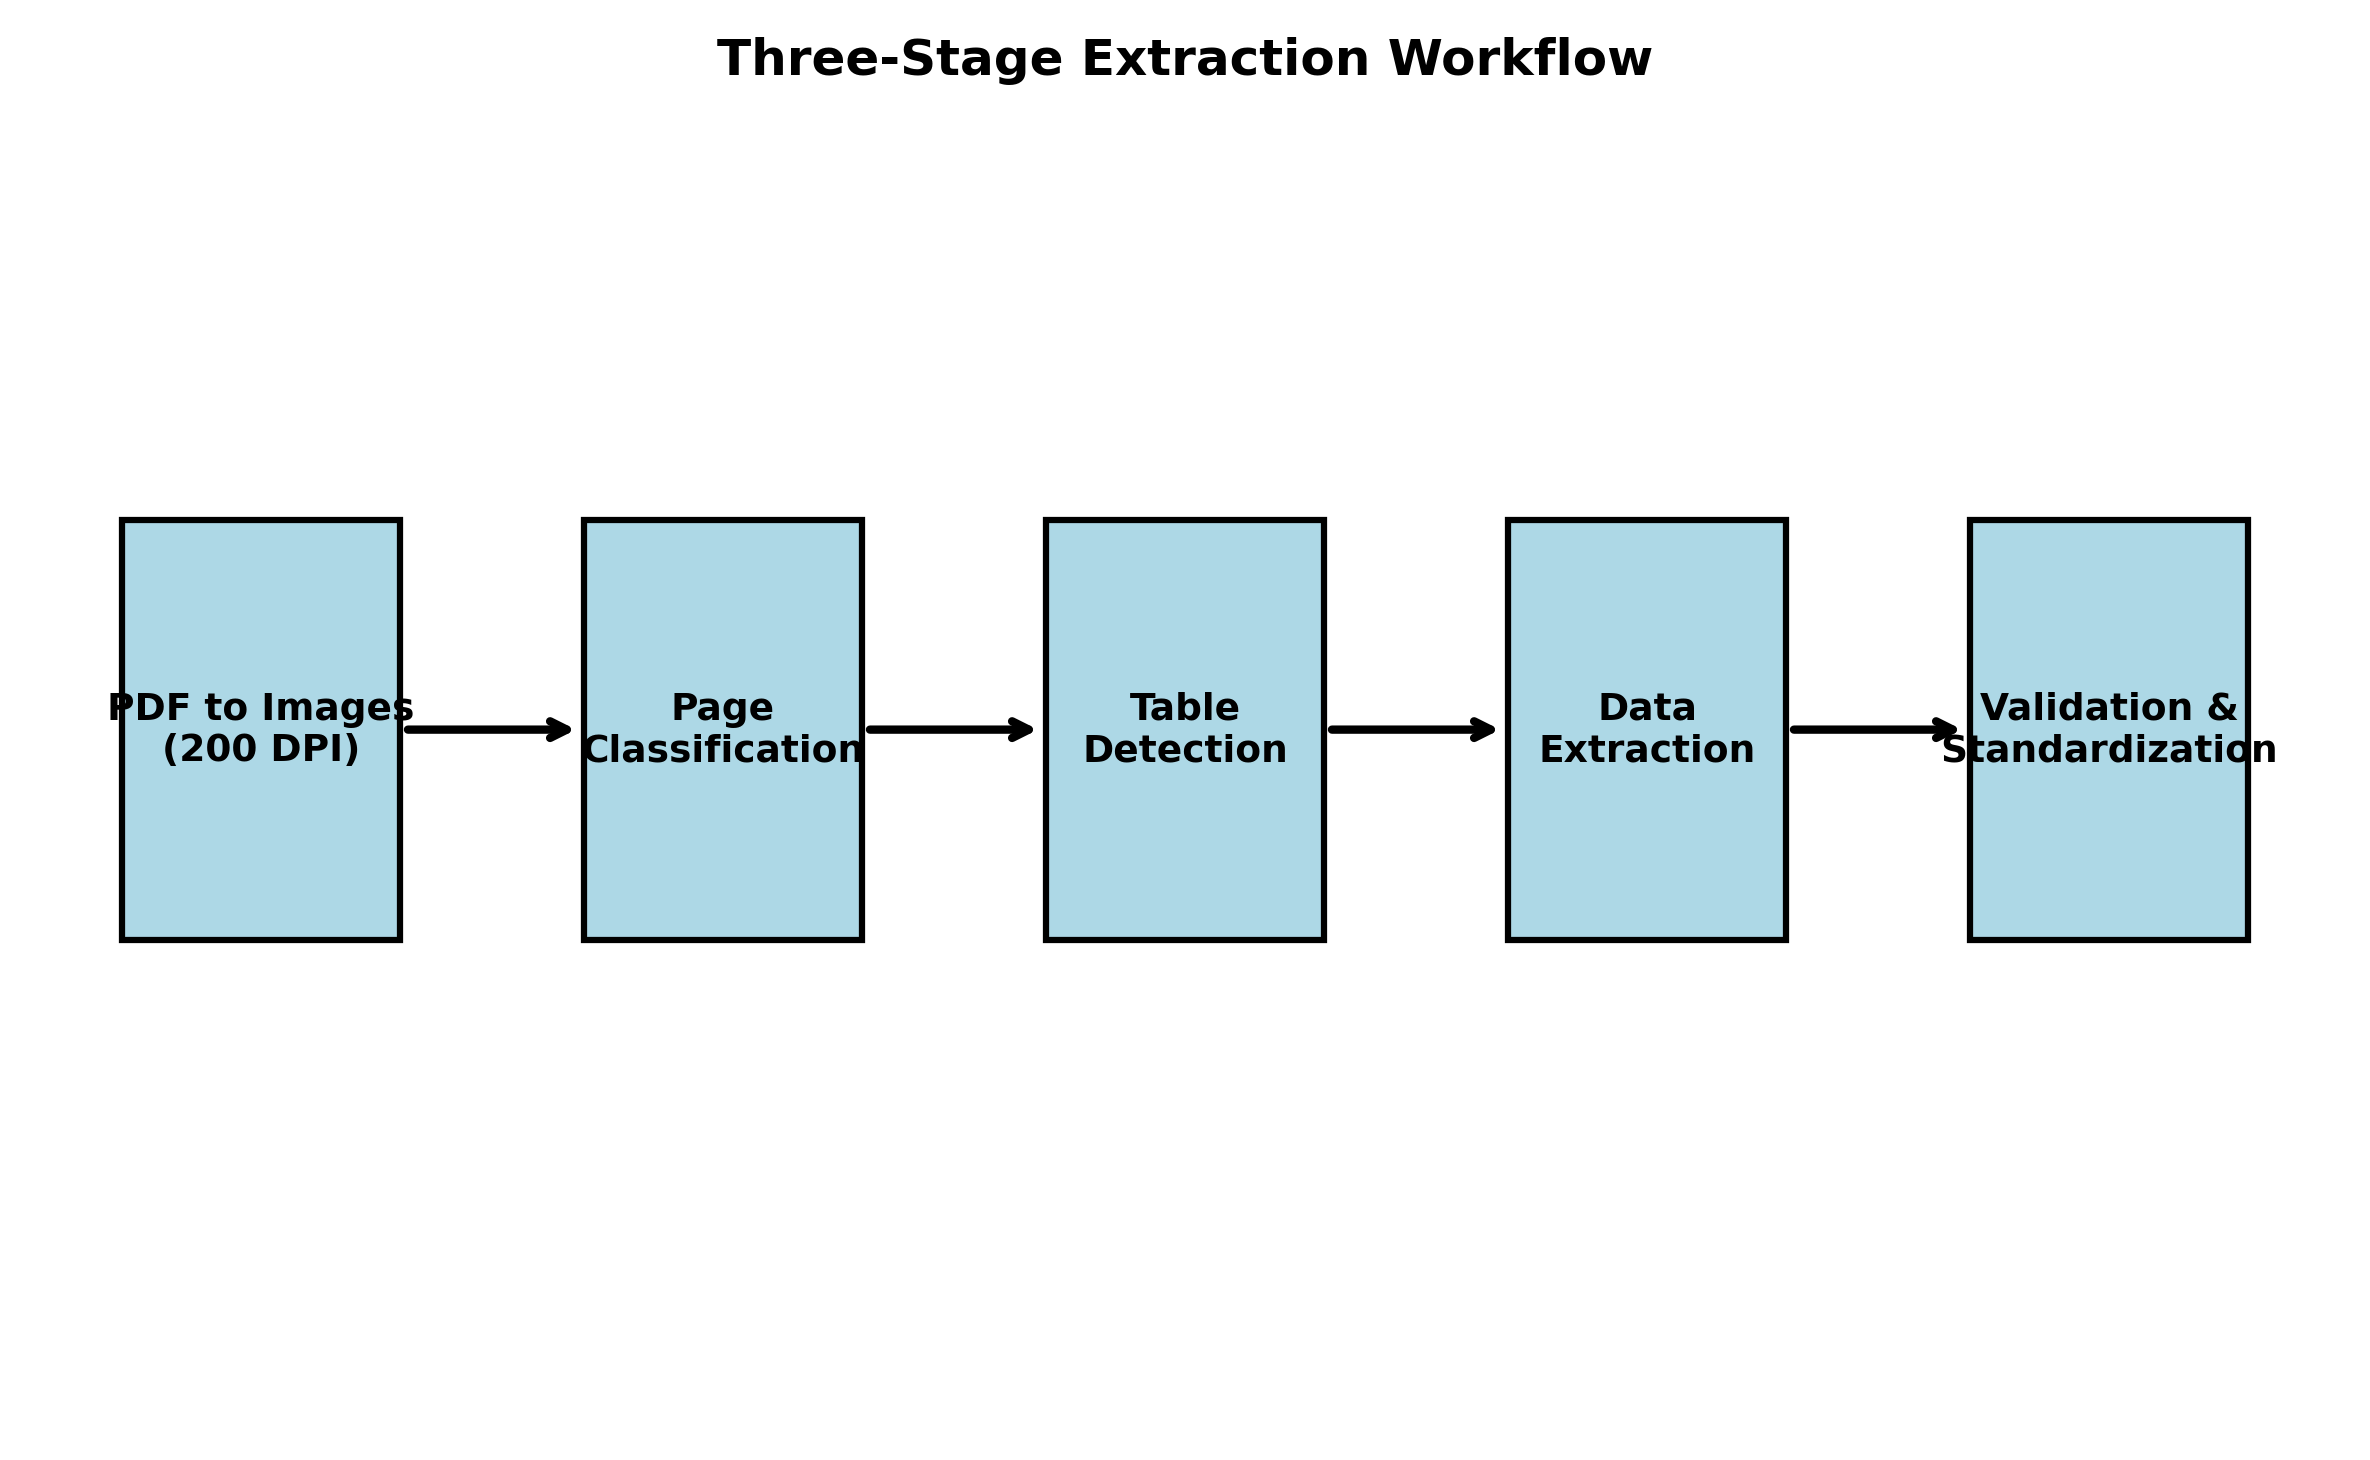
\includegraphics[width=\columnwidth]{fig6_workflow.png}}
\caption{Extraction workflow pipeline.}
\label{fig:workflow}
\end{figure}

\subsection{Experimental Design}

\textbf{Model Comparison:} A 63-page report with 28 data tables was processed using all four architectures with identical prompts. Metrics included processing time, classification accuracy, row completeness, and GPU utilization.

\textbf{Bulk Processing:} The best-performing model processed all 15 reports to evaluate production stability, success rate, and computational requirements.

\textbf{Prompt Strategy Comparison:} Baseline and quality control prompts were compared to isolate prompt engineering effects on accuracy versus cost. Manual validation quantified classification error rates.

Hardware included NVIDIA RTX 6000 (48 GB) for primary processing and Tesla L4 (22 GB) for validation. All experiments used PyTorch 2.5.1 with CUDA 12.1 on Ubuntu 22.04 LTS.

\subsection{Data Consolidation Methodology}

Historical outputs from 94 CSV files were consolidated into unified datasets. Column names (2,856 variants) were normalized through lowercase conversion, whitespace standardization, and semantic grouping based on domain knowledge. A unified schema mapped variants to 147 standardized patterns. Rows were merged with source tracking, numeric columns detected automatically, and invalid ranges removed.

\section{Results}

\subsection{Model Performance Comparison}

Comparing the four architectures revealed stark performance differences (Table~\ref{tab:model_comparison}, Fig.~\ref{fig:model_performance}). The olmOCR-2-7B model completed processing in just 36 minutes while extracting all 160 ground truth rows. In contrast, the Qwen3-VL-4B took 81 minutes but captured only 76 rows due to excessive hallucination. The 30B model exceeded 3 hours before termination, proving impractical despite its theoretical advantages. These results position olmOCR as the clear winner for production deployment.

\begin{table}[htbp]
\caption{Model Performance on 63-Page Test Report}
\label{tab:model_comparison}
\begin{center}
\small
\begin{tabular}{lcccc}
\toprule
\textbf{Metric} & \textbf{4B} & \textbf{8B} & \textbf{30B} & \textbf{olmOCR} \\
\midrule
Runtime (min) & 81 & 150 & >180 & 36 \\
Rows Extracted & 76 & 120 & - & 160 \\
Classification Accuracy & Low & Medium & - & High \\
Completeness & 48\% & 75\% & - & 100\% \\
\bottomrule
\end{tabular}
\end{center}
\end{table}

\begin{figure}[htbp]
\centerline{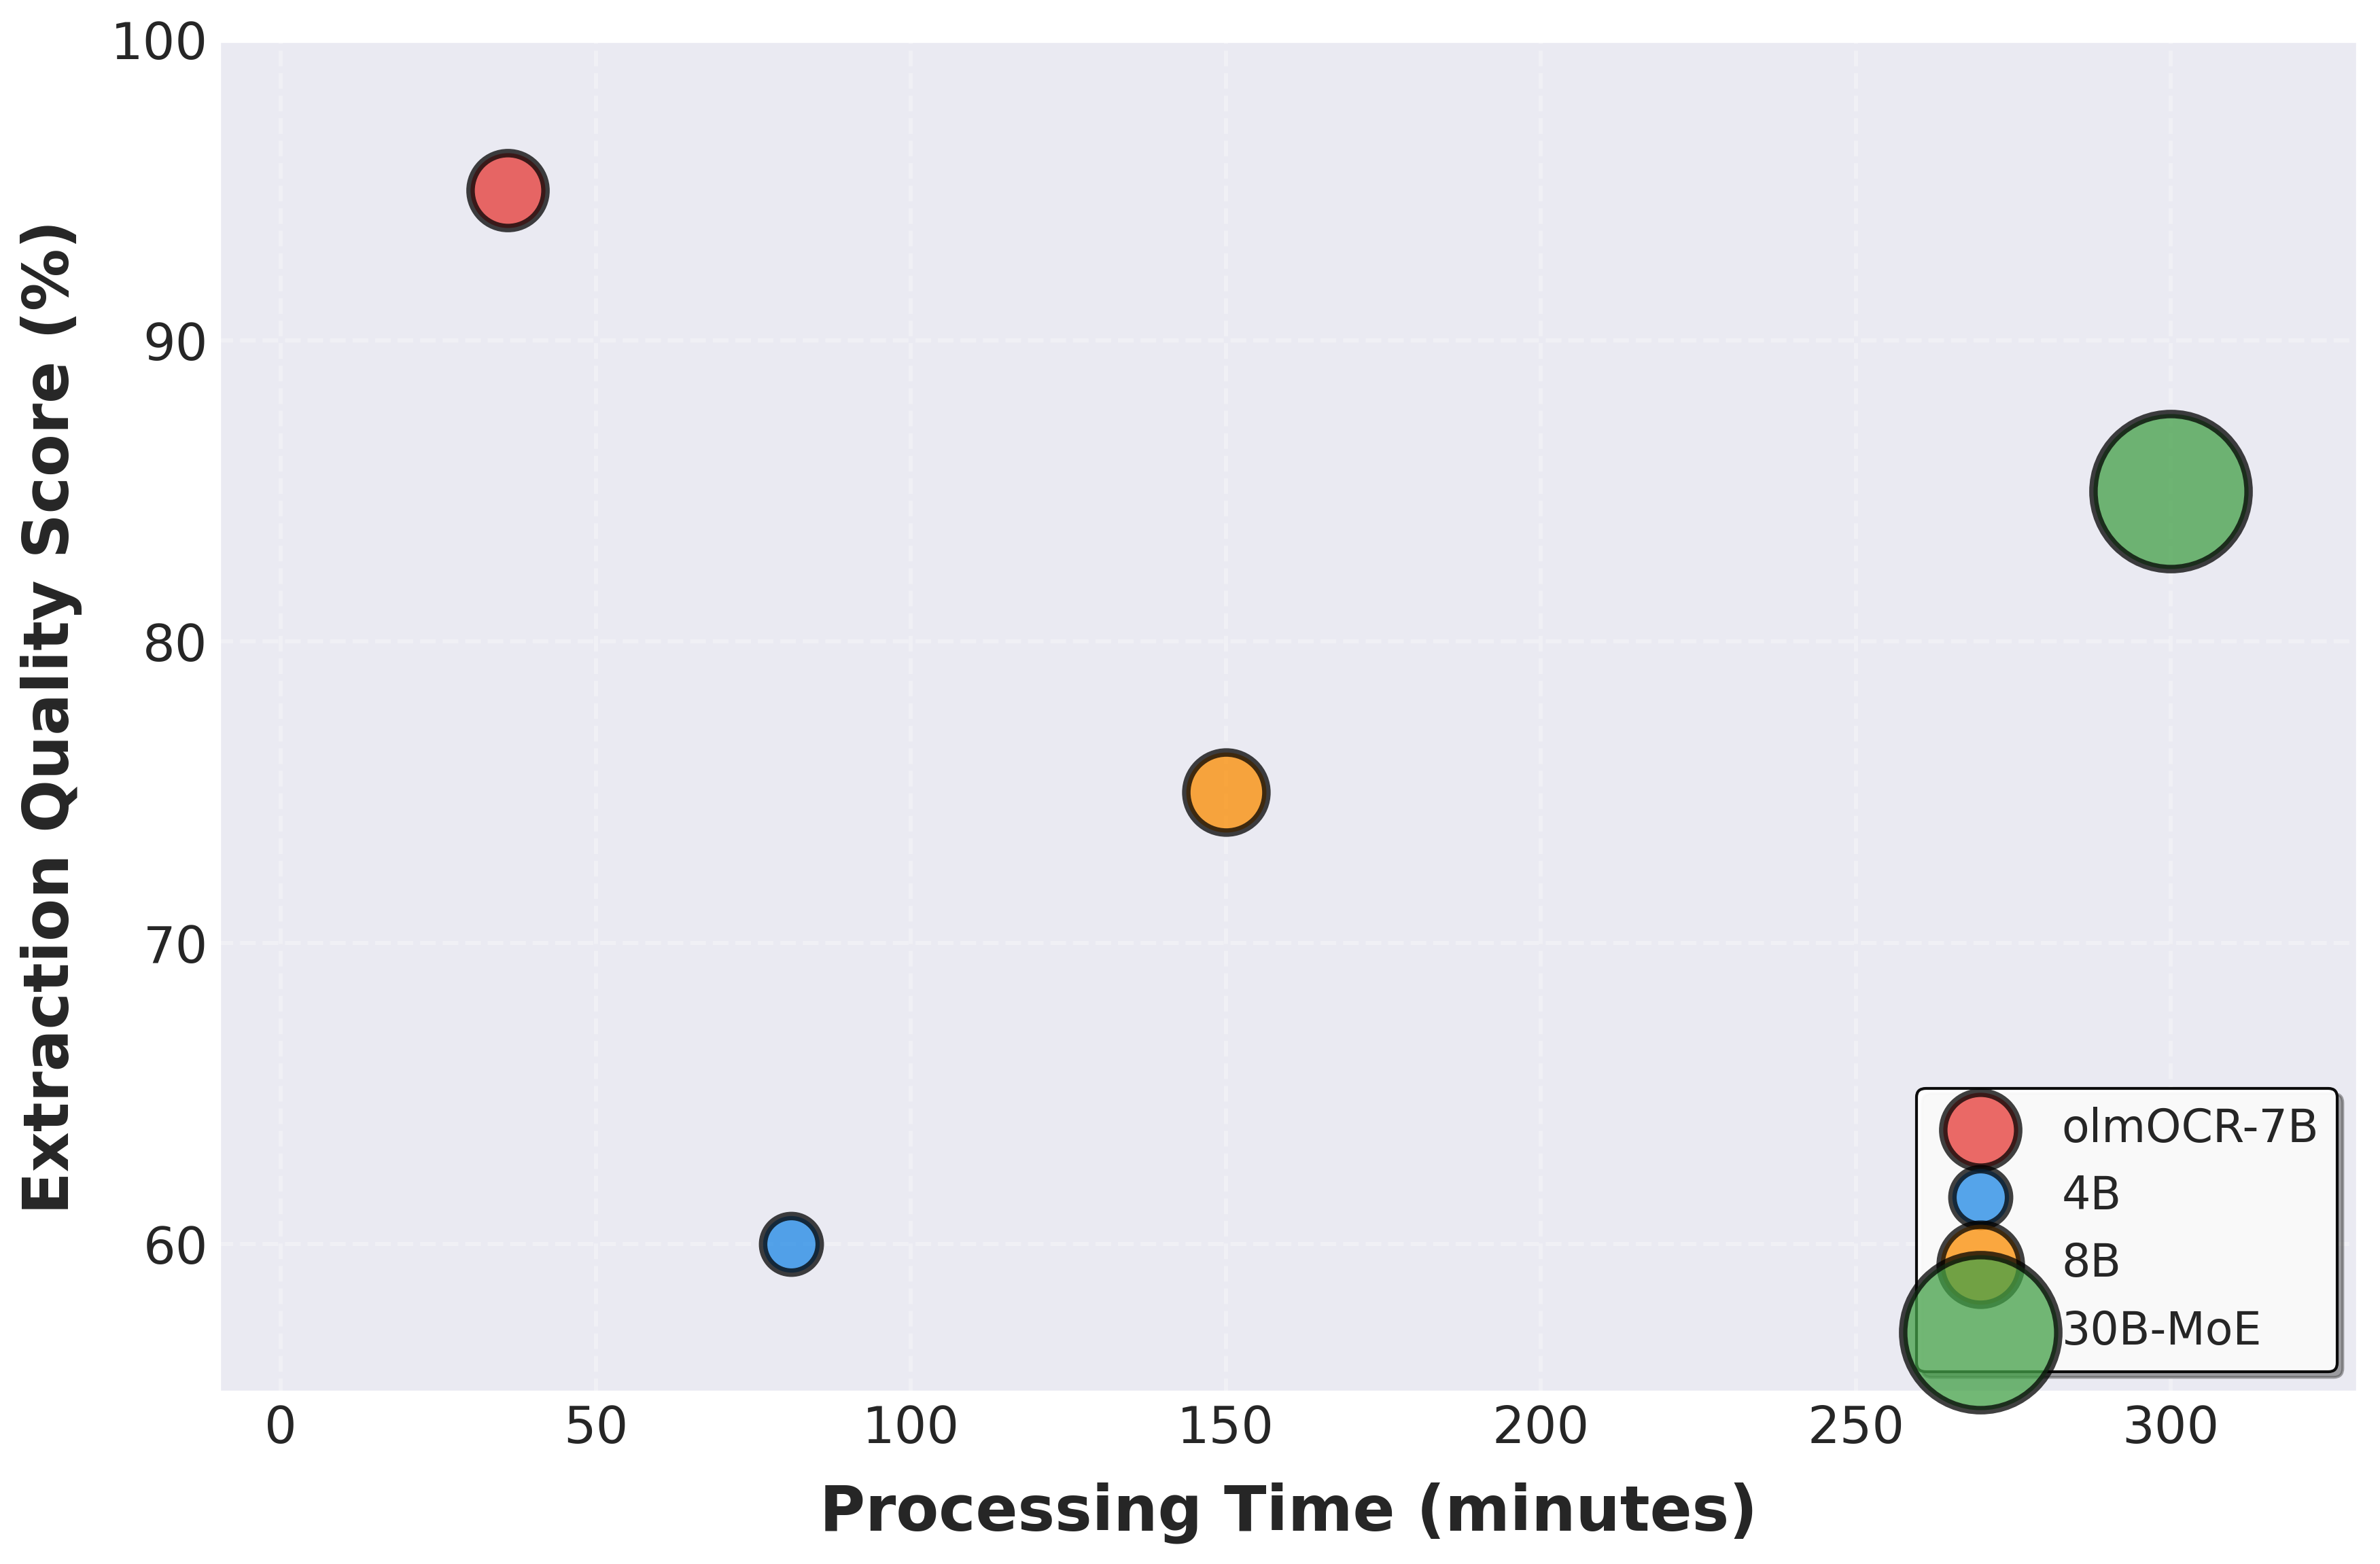
\includegraphics[width=0.8\columnwidth]{fig1_model_performance.png}}
\caption{Model performance tradeoffs (bubble size indicates capacity).}
\label{fig:model_performance}
\end{figure}

The performance landscape shows that smaller models sacrifice accuracy for speed while the largest model imposes prohibitive costs. The 7B olmOCR architecture occupies the sweet spot, delivering both high quality and practical runtime.

\subsection{Large-Scale Processing Results}

Scaling to all 15 reports, olmOCR achieved perfect reliability (Table~\ref{tab:bulk_results}). Total processing required 26 hours with an average of 104 minutes per report. The largest document (421 pages) took 14.6 hours while the smallest (17 pages) finished in 6.7 minutes. This linear scaling relationship (2.08 minutes per page) enables accurate capacity planning for production deployments.

\begin{table}[htbp]
\caption{Bulk Processing Summary (15 Reports)}
\label{tab:bulk_results}
\begin{center}
\small
\begin{tabular}{lc}
\toprule
\textbf{Metric} & \textbf{Result} \\
\midrule
Total pages processed & 1,374 \\
Total tables extracted & 691 \\
Total rows extracted & 3,778 \\
Processing time & 1,562 min \\
Average time per page & 1.14 min \\
Success rate & 100\% \\
\bottomrule
\end{tabular}
\end{center}
\end{table}

Page type distribution across all documents (Fig.~\ref{fig:page_distribution}) confirmed that data tables dominate at 50.3\%, validating our focus on table extraction. GPU memory remained stable at 15.45 GB throughout, enabling concurrent processing on high-capacity hardware.

\begin{figure}[htbp]
\centerline{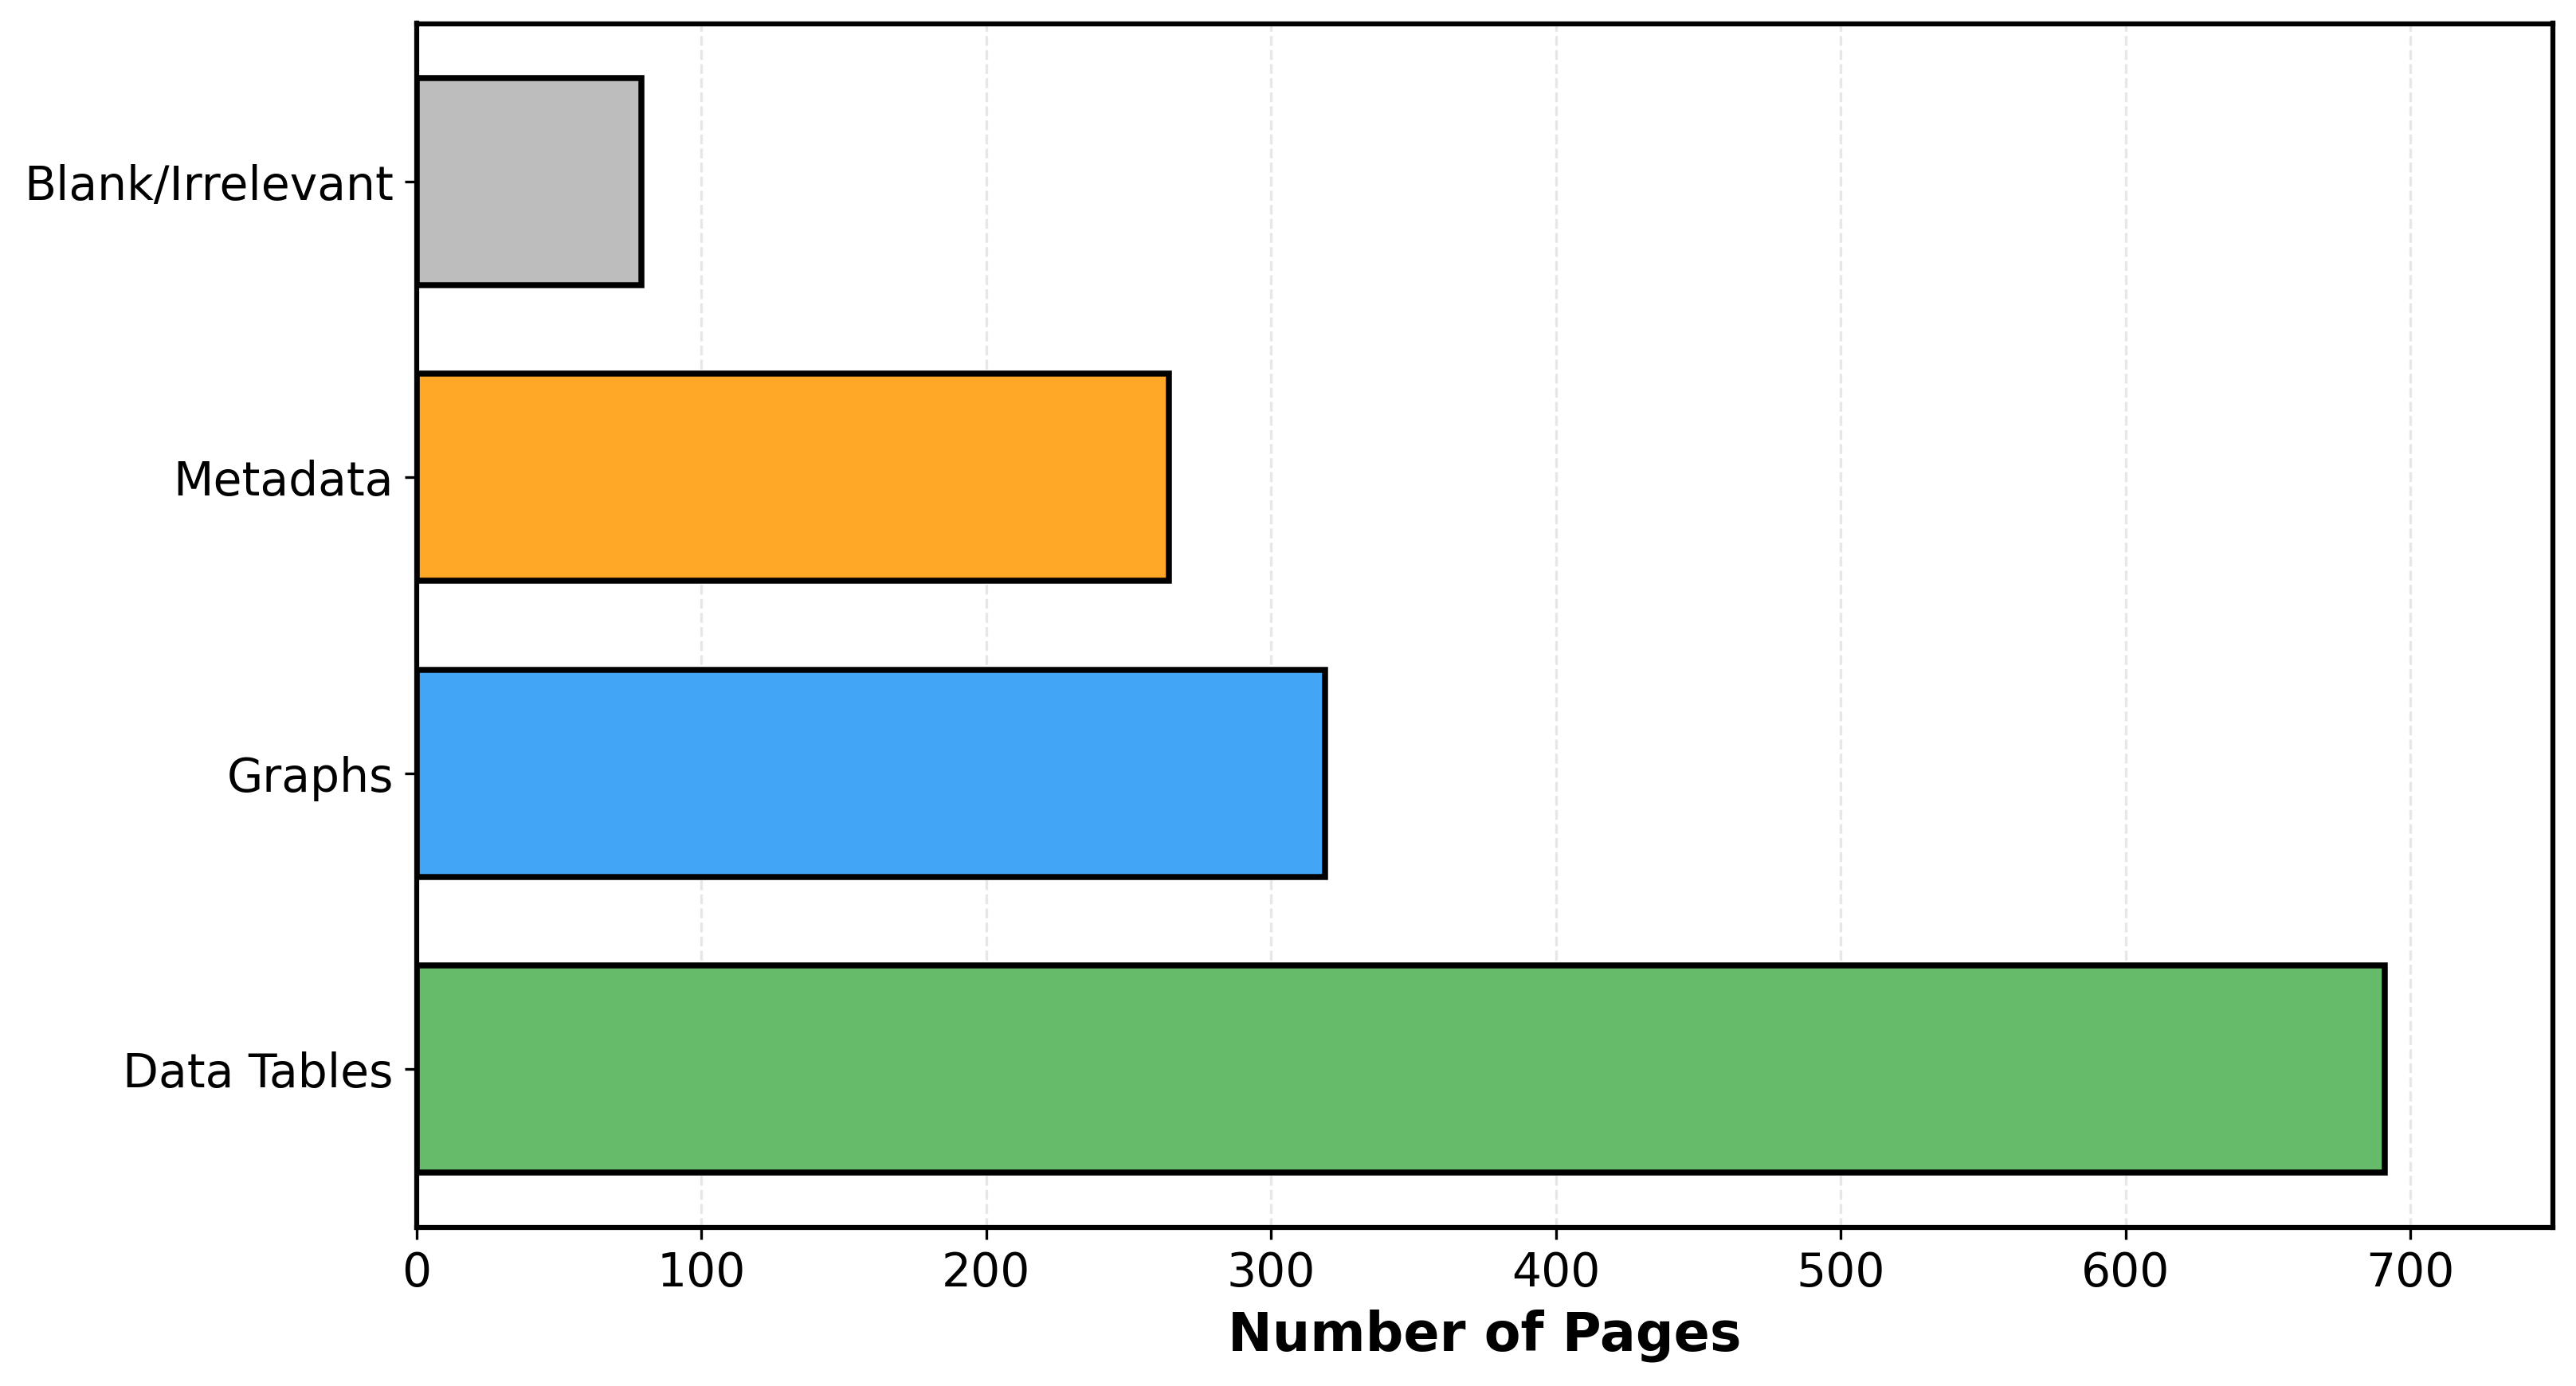
\includegraphics[width=0.8\columnwidth]{fig2_page_distribution.png}}
\caption{Page type distribution across 1,374 pages.}
\label{fig:page_distribution}
\end{figure}

Processing time scaled linearly with document size (Fig.~\ref{fig:scalability}, R² = 0.92), demonstrating predictable resource requirements across the entire corpus.

\begin{figure}[htbp]
\centerline{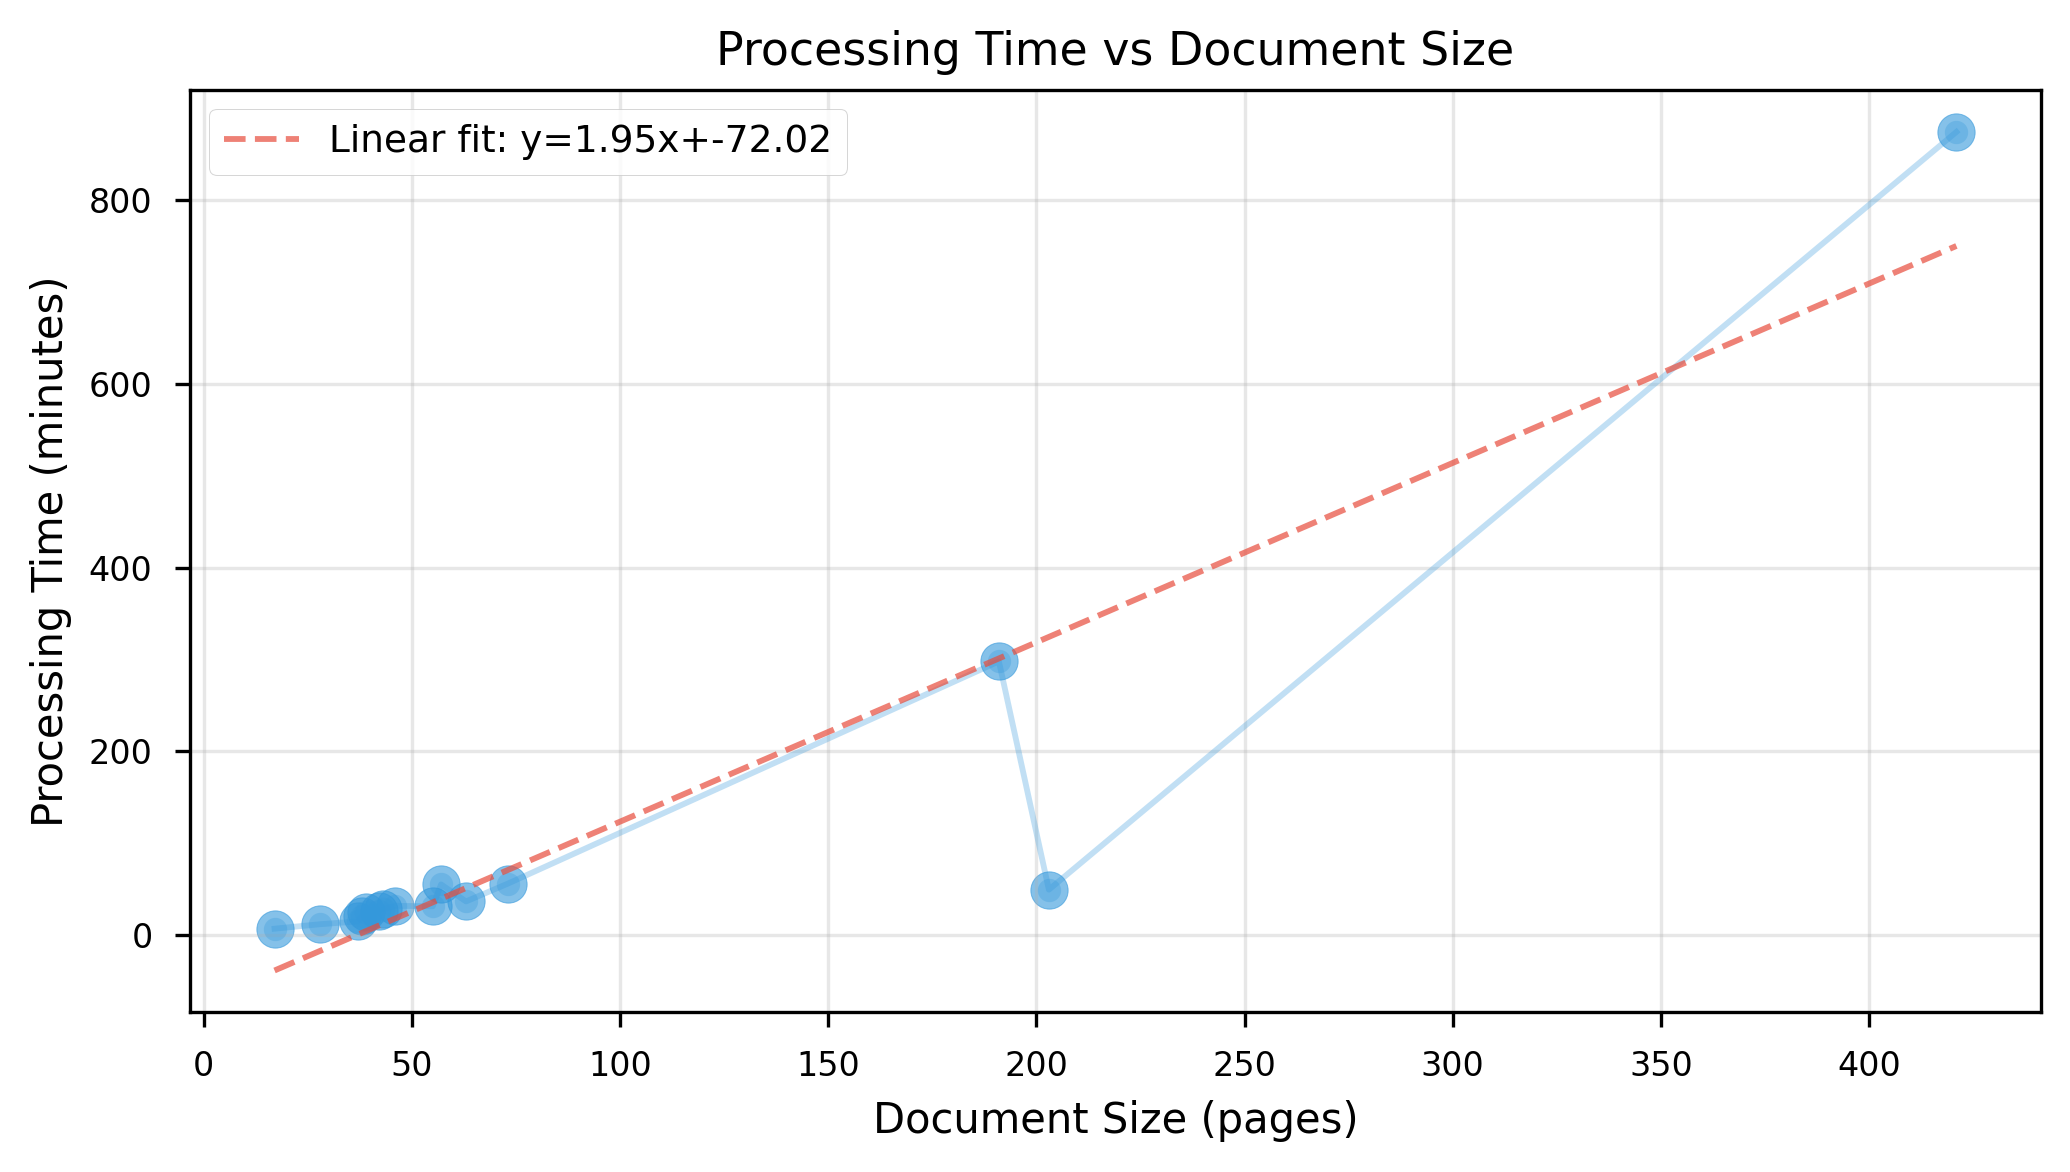
\includegraphics[width=0.8\columnwidth]{fig5_scalability.png}}
\caption{Linear scaling at 2.08 min/page (R² = 0.92).}
\label{fig:scalability}
\end{figure}

\subsection{Prompt Engineering Impact}

Quality control prompting transformed accuracy but at substantial computational cost (Table~\ref{tab:qc_comparison}, Fig.~\ref{fig:prompt_comparison}). The baseline prompt misclassified 43\% of pages, incorrectly categorizing graphs as metadata and extracting 130 hallucinated rows from axis labels. Enhanced prompting eliminated all errors through strict validation criteria but required 280 minutes versus 36 minutes baseline—a 7.8-fold increase.

\begin{table}[htbp]
\caption{Baseline vs Quality Control Prompt Comparison}
\label{tab:qc_comparison}
\begin{center}
\small
\begin{tabular}{lcc}
\toprule
\textbf{Metric} & \textbf{Baseline} & \textbf{QC Enhanced} \\
\midrule
Runtime (min) & 36 & 280 \\
Classification errors & 27/63 (43\%) & 0/63 (0\%) \\
Hallucinated rows & 130 & 0 \\
Column naming & Raw variants & Standardized \\
\bottomrule
\end{tabular}
\end{center}
\end{table}

\begin{figure}[htbp]
\centerline{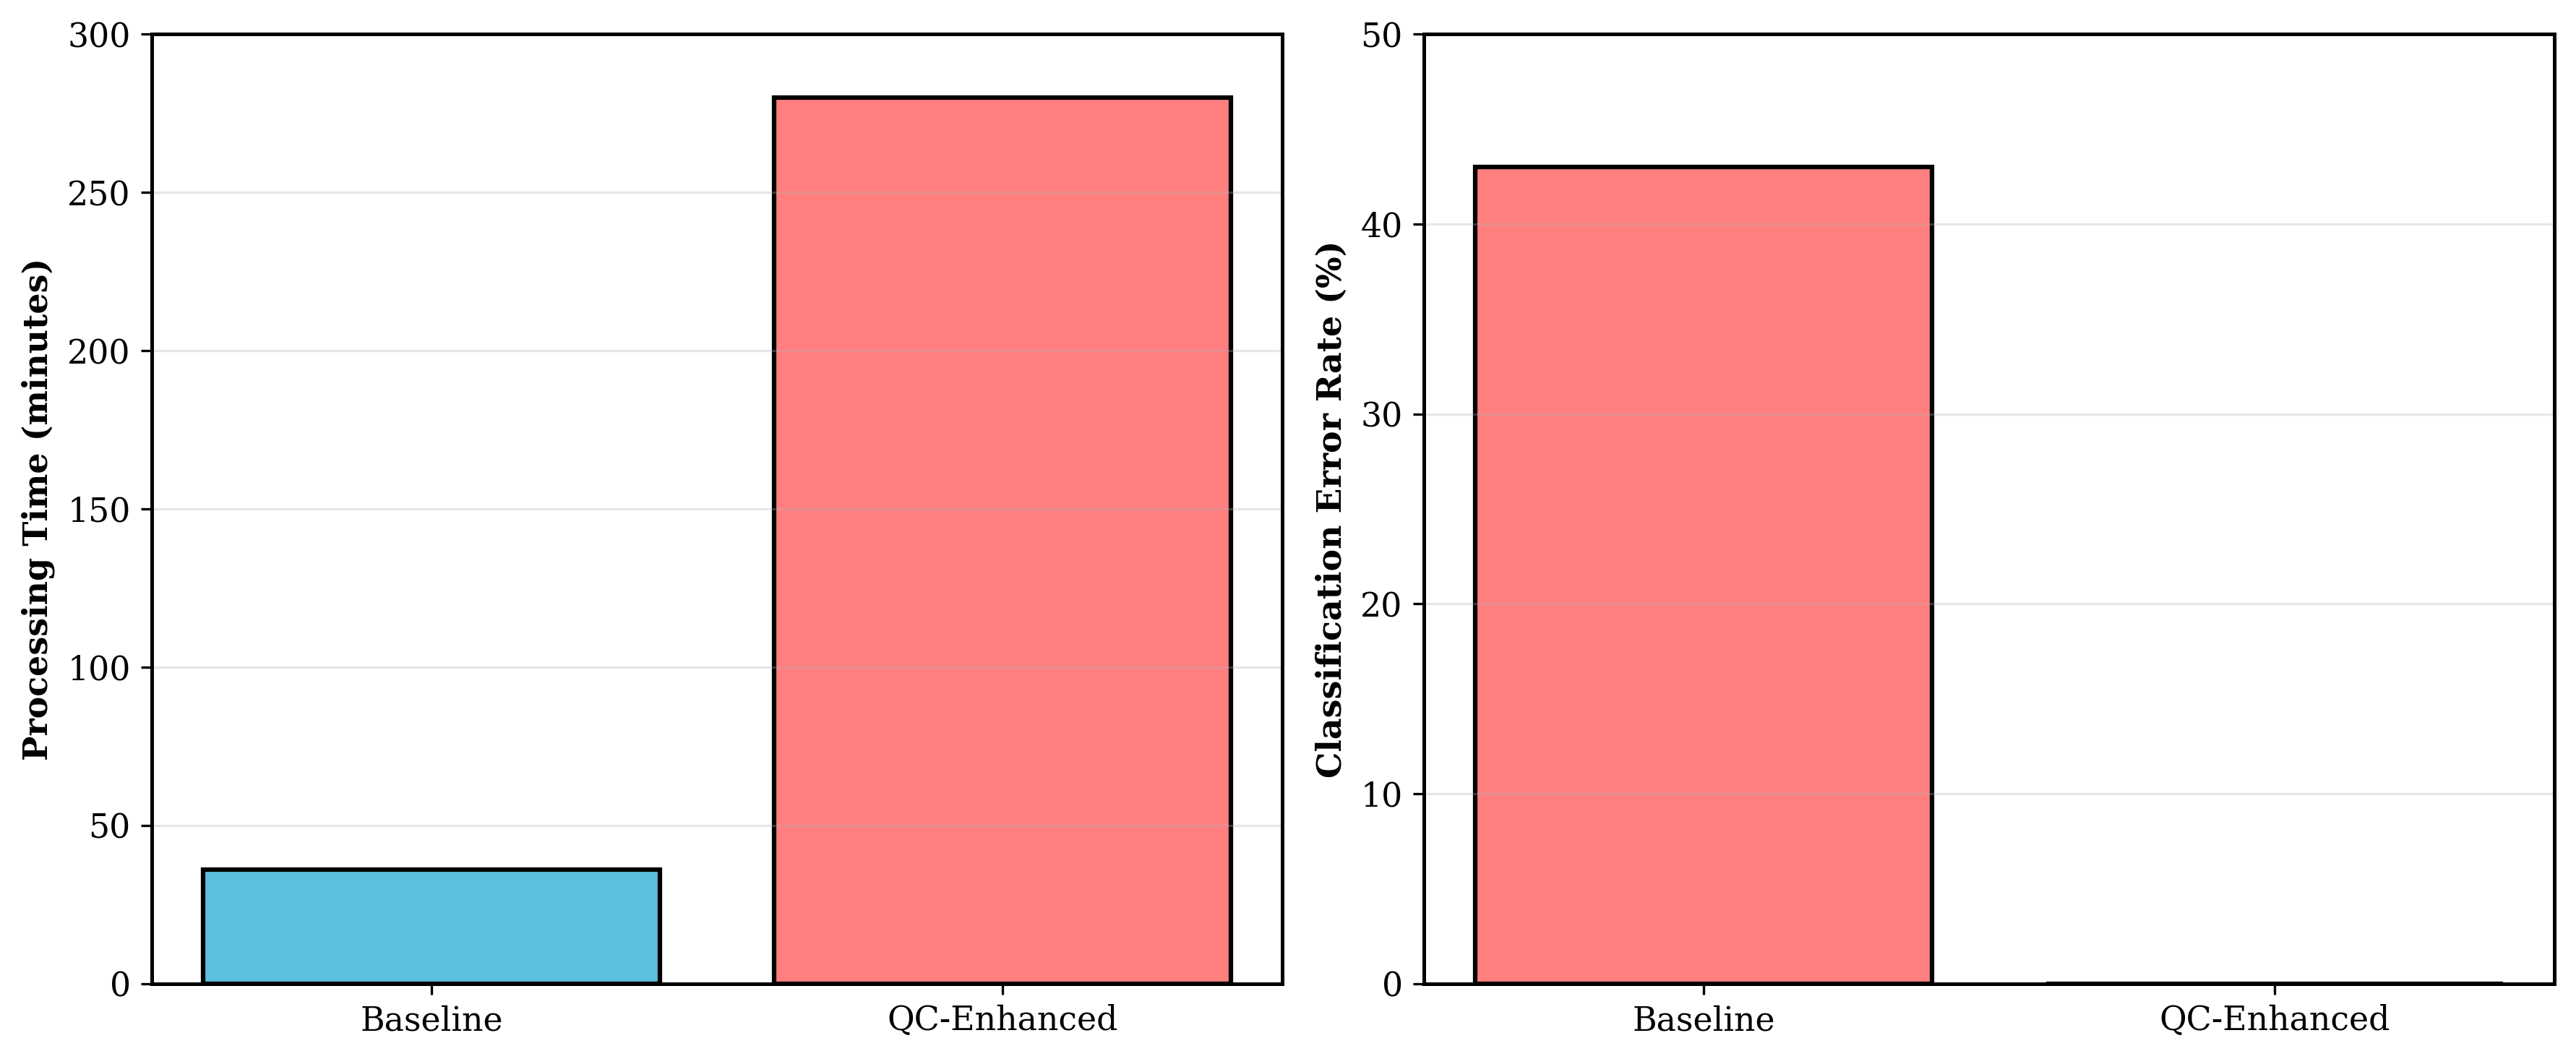
\includegraphics[width=\columnwidth]{fig3_prompt_comparison.png}}
\caption{Accuracy-efficiency tradeoff in prompt strategies.}
\label{fig:prompt_comparison}
\end{figure}

This fundamental tradeoff requires careful consideration for production deployment. Organizations must balance accuracy requirements against computational budgets.

\subsection{Structural Analysis}

General extraction without classification assumptions revealed remarkable diversity (Table~\ref{tab:general_extraction}). We identified 547 distinct table structures with 1-17 columns and varying semantic categories. This heterogeneity confirms that universal extraction strategies cannot optimize across all table types. Domain-specific approaches targeting known structures achieve superior results.

\begin{table}[htbp]
\caption{General Extraction Structural Analysis}
\label{tab:general_extraction}
\begin{center}
\small
\begin{tabular}{lc}
\toprule
\textbf{Metric} & \textbf{Result} \\
\midrule
Total tables identified & 547 \\
Column range per table & 1--17 \\
Median columns & 6 \\
Processing time & 1,020 min \\
\bottomrule
\end{tabular}
\end{center}
\end{table}

\subsection{Data Consolidation Outcomes}

Consolidating historical extractions produced unified machine learning-ready datasets (Table~\ref{tab:consolidation}). Processing 94 CSV files reduced 2,856 column name variants to 147 normalized patterns through systematic text processing and semantic grouping (Fig.~\ref{fig:consolidation}). The final dataset contained 16,834 rows after removing 110 duplicates.

\begin{table}[htbp]
\caption{Data Consolidation Results}
\label{tab:consolidation}
\begin{center}
\small
\begin{tabular}{lc}
\toprule
\textbf{Metric} & \textbf{Result} \\
\midrule
Input CSV files & 94 \\
Raw column variants & 2,856 \\
Final normalized patterns & 147 \\
ML-ready rows & 16,834 \\
Duplicates removed & 110 \\
\bottomrule
\end{tabular}
\end{center}
\end{table}

\begin{figure}[htbp]
\centerline{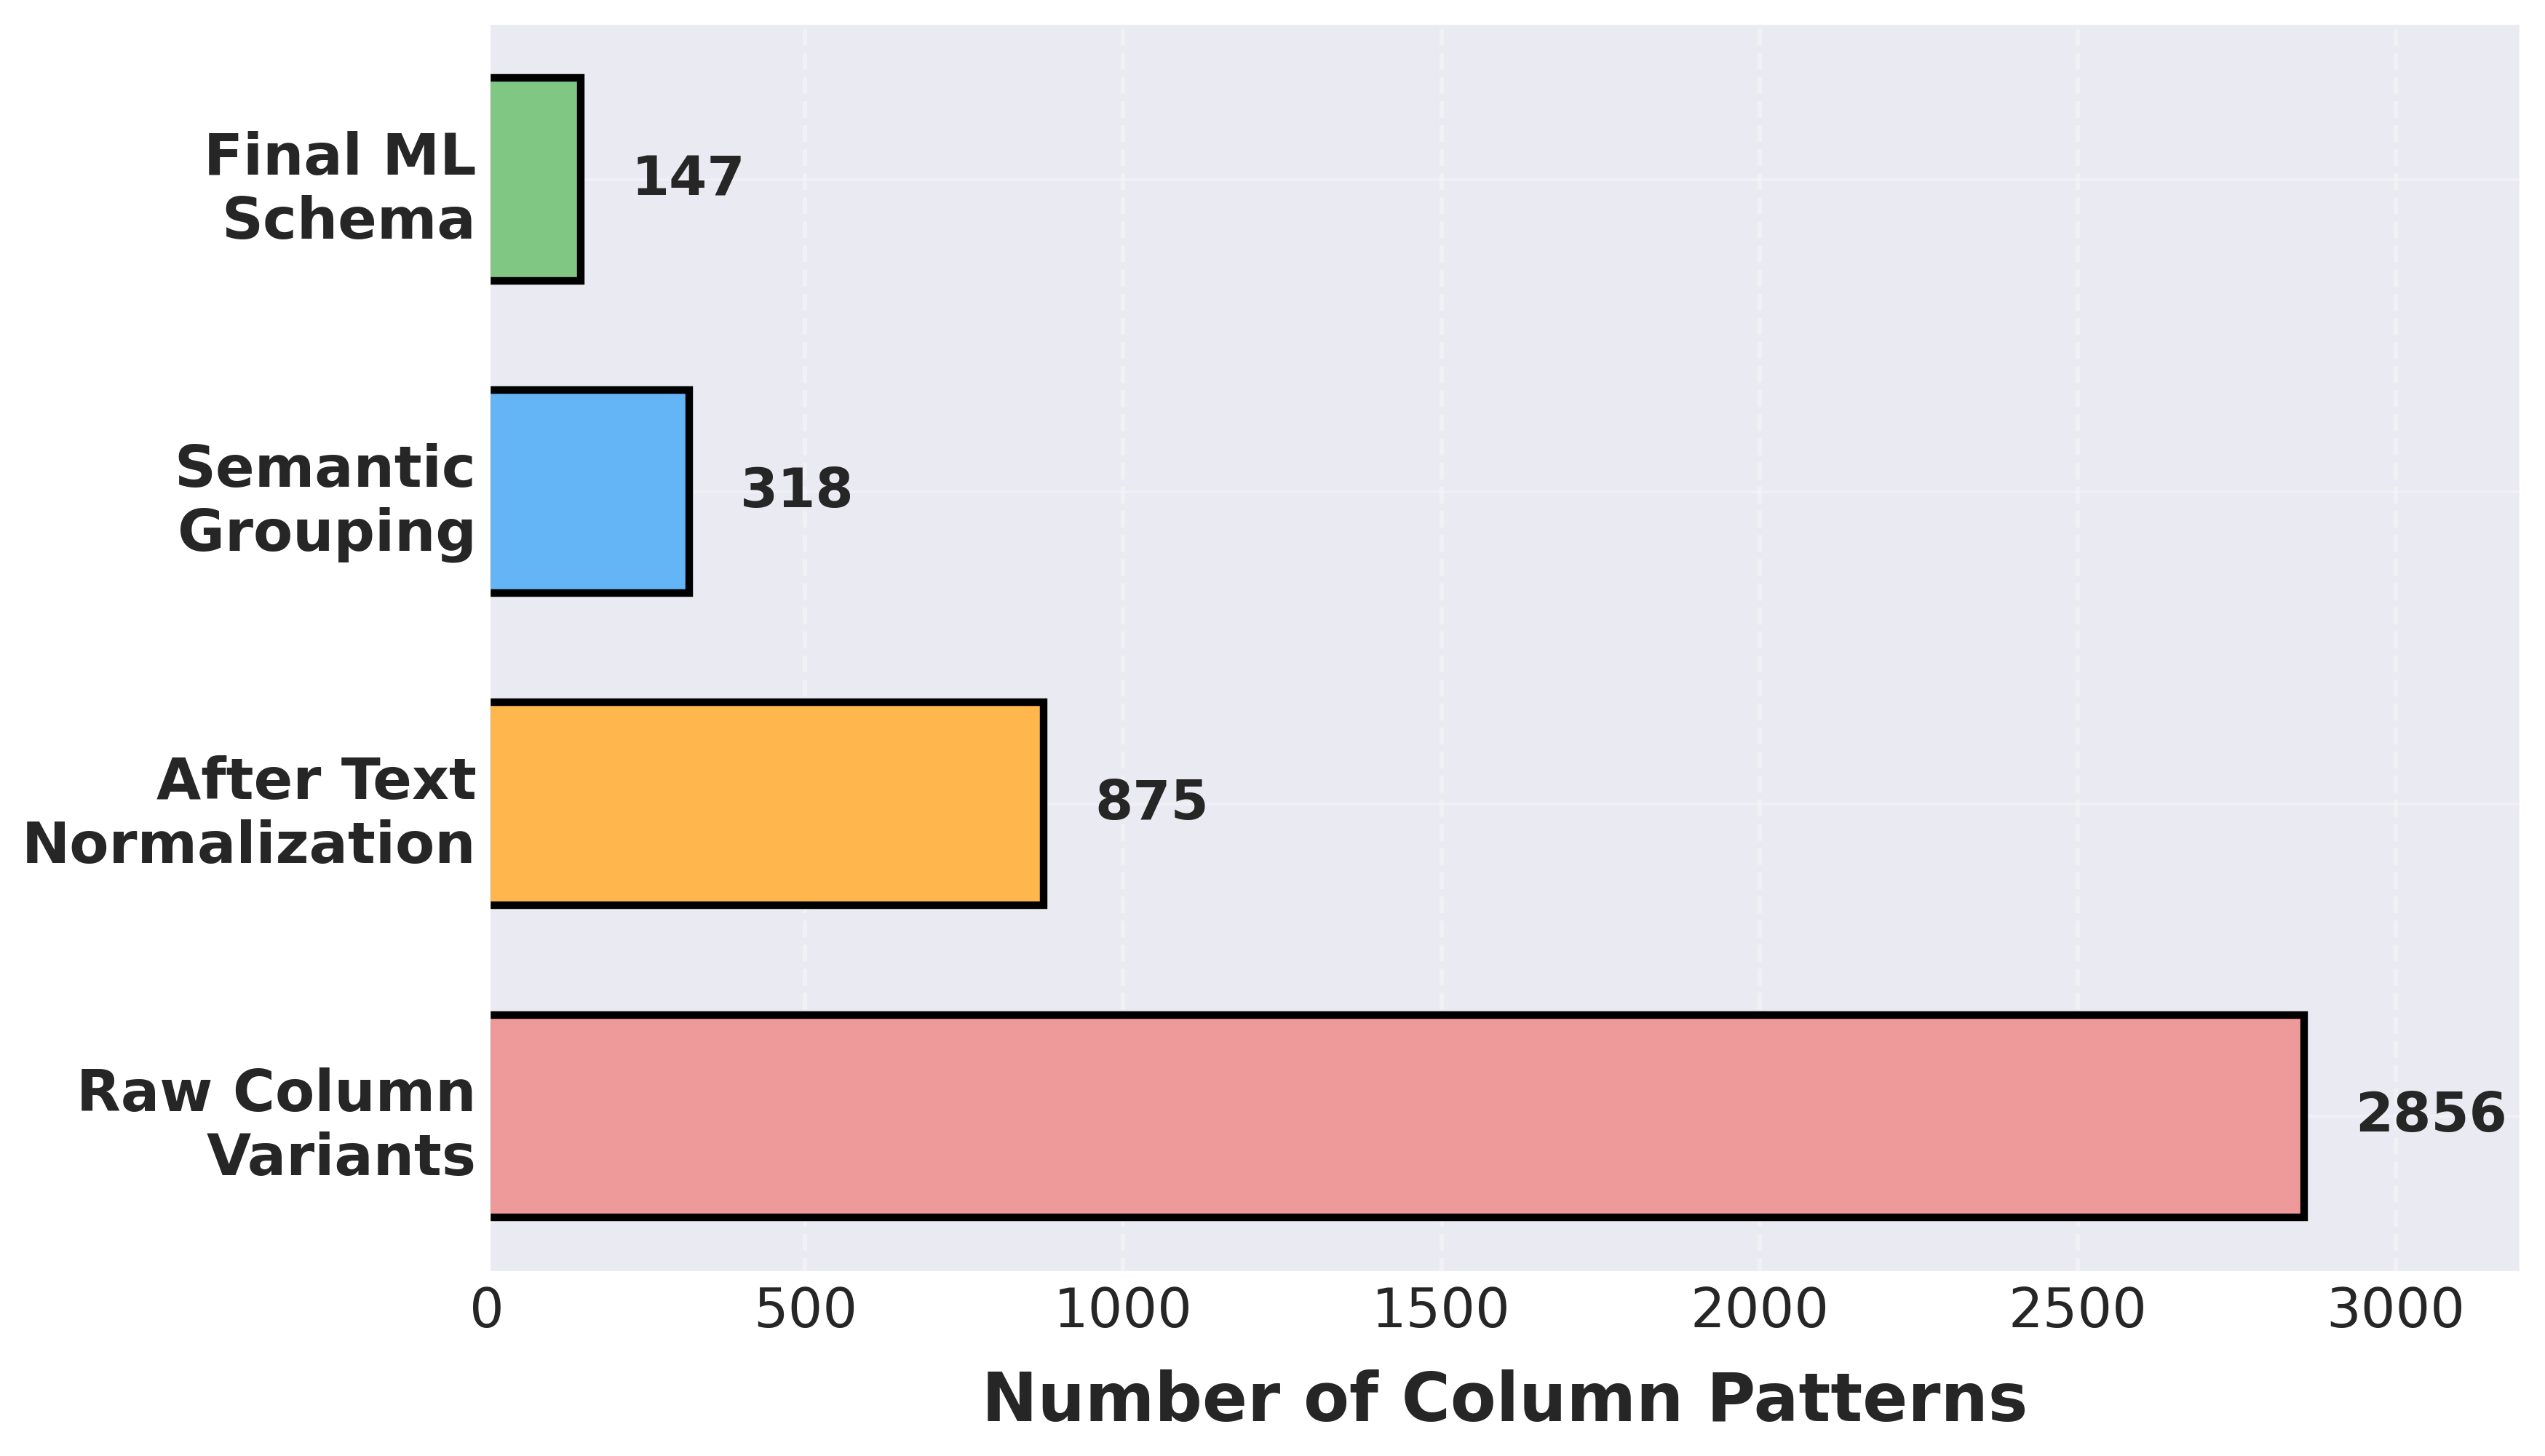
\includegraphics[width=0.8\columnwidth]{fig4_consolidation.png}}
\caption{Progressive column variant reduction.}
\label{fig:consolidation}
\end{figure}

While deterministic text processing handled syntactic variations, semantic variants required domain knowledge. Abbreviations like "CPOR", "He Porosity", and "Phi\_He" all represent identical measurements but need expert mapping to unify correctly.

\section{Discussion}

\subsection{Model Selection for Production}

The olmOCR-2-7B model emerged as optimal for production deployment, balancing accuracy and efficiency effectively. Specialized fine-tuning for OCR tasks contributed to superior performance on technical measurements with units and precision requirements \cite{e2e2025}. While the 30B mixture-of-experts architecture offers theoretical advantages, impractical runtimes preclude operational use. The 4B variant exhibited unacceptable hallucination requiring extensive manual correction.

Mid-sized architectures (7-8B parameters) with domain-specific tuning outperform generic large models for document understanding. This aligns with recent literature showing specialized smaller models beat general-purpose larger ones for focused applications \cite{yang2024}.

\subsection{Accuracy-Efficiency Tradeoff}

The 7.8-fold runtime increase from quality control prompting quantifies a fundamental tension between accuracy and cost. Three operational strategies emerge:

\textbf{High-accuracy mode} deploys quality control prompts with extended runtime for critical data requiring zero error tolerance.

\textbf{Balanced mode} employs baseline prompts with post-processing validation to flag potential errors for human review, optimizing automation-expert division of labor.

\textbf{High-throughput mode} uses simplified prompts targeting known structures, sacrificing generality for speed in reconnaissance-level extraction.

Strategy selection depends on downstream error sensitivity, computational resources, and labor costs for validation.

\subsection{Implications of Format Heterogeneity}

Identifying 547 distinct table structures across just 15 reports demonstrates substantial format diversity stemming from different vendors, evolving standards, and sample-specific customization. This validates focusing on use-case-driven extraction rather than universal approaches.

Target applications typically need only 2-3 specific table types per report. Focused workflows achieve superior accuracy with reduced cost compared to general extraction. Production systems should classify table types first, then route to specialized extraction prompts optimized for specific structures.

\subsection{Consolidation Challenges}

Reducing 2,856 column variants to 147 patterns reveals substantial naming inconsistency. Beyond syntactic variations, semantic variants require domain knowledge. Abbreviation expansion, unit standardization, and property synonyms all need expert knowledge or comprehensive ontologies.

The 1.6\% overlap between historical and PDF extractions indicates largely non-overlapping sources, constraining validation coverage. Future work should construct validation datasets with manual annotation across representative samples.

\subsection{Computational Feasibility at Scale}

The 26-hour processing time for 15 reports establishes baseline computational requirements. Scaling to institutional archives requires parallel processing infrastructure, efficient job scheduling, and incremental processing capabilities. Stable 15.45 GB VRAM utilization enables concurrent execution on high-capacity GPUs. Four NVIDIA A100 GPUs (80 GB each) could process 100 reports in 12 hours with proper load balancing.

\subsection{Comparison with Manual Extraction}

Industry experience indicates manual transcription requires 4-8 hours per report \cite{schilling2024}. Our automated system averages 1.7 hours per report, representing 2.4-4.7× speed improvement. However, this excludes downstream validation time. The crossover point where automated extraction plus validation beats pure manual transcription appears around 10-15 report batches where setup costs amortize.

\subsection{Limitations and Future Directions}

Several constraints limit generalizability. The 15-report dataset may not fully represent global documentation variations across domains and time periods. Focus on English leaves multilingual performance unvalidated despite theoretical multilingual capabilities \cite{wen2023}. VLM architectures evolve rapidly, potentially altering performance characteristics. Manual validation covered representative samples but comprehensive ground truth for all 3,778 rows was not established.

Future research should explore hybrid workflows combining rapid general extraction with targeted high-accuracy extraction for critical fields. Active learning leveraging human corrections can fine-tune models for domain-specific layouts. Multimodal validation incorporating graph analysis can cross-validate tabular data against plots. Distributed processing frameworks enable production-scale throughput.

\section{Conclusion}

This investigation demonstrates technical viability of VLM-based automation for scientific document extraction while revealing critical tradeoffs. The olmOCR-2-7B architecture achieved 100\% processing success across 15 heterogeneous reports, extracting 3,778 data rows in 104 minutes per document average. Quality control prompting eliminated classification errors entirely at 7.8× computational cost, quantifying the fundamental accuracy-efficiency tension.

We identified 547 distinct table structures, validating use-case-driven extraction over universal approaches. Consolidation produced machine learning-ready datasets with 16,834 rows by mapping 2,856 column variants to 147 normalized patterns through systematic schema discovery.

Key findings for practitioners: prioritize mid-sized architectures (7-8B parameters) with domain-specific fine-tuning over generic large models; align prompt complexity with accuracy requirements and computational constraints; incorporate domain knowledge for semantic unification beyond syntactic normalization.

Future work should explore hybrid human-machine workflows, active learning for continuous improvement, and distributed processing for institutional-scale deployment. This methodology provides foundation for intelligent document processing in scientific and technical domains.

\section*{Acknowledgment}

This research was conducted at the Faculty of Computing and Informatics, Universiti Malaysia Sabah. The authors thank laboratory personnel for providing access to technical report archives.

\begin{thebibliography}{20}

\bibitem{carolan2024}
K. Carolan, L. Fennelly, and A. Smeaton, ``A Review of Multi-Modal Large Language and Vision Models,'' arXiv preprint arXiv:2404.01322, 2024.

\bibitem{huang2024}
D. Huang, C. Yan, Q. Li, and X. Peng, ``From Large Language Models to Large Multimodal Models: A Literature Review,'' \textit{Appl. Sci.}, vol. 14, no. 12, p. 5068, 2024.

\bibitem{bansal2025}
R. Bansal, B. Shah, A. Chanda, and V. Parate, ``Optimizing PDF Ingestion for Large Language Models in RAG Architectures,'' \textit{Int. J. Appl. Math.}, vol. 38, no. 3, 2025.

\bibitem{bai2024}
T. Bai, H. Liang, B. Wan, L. Yang, B. Li, Y. Wang, B. Cui, C. He, B. Yuan, and W. Zhang, ``A Survey of Multimodal Large Language Model from A Data-centric Perspective,'' arXiv preprint arXiv:2405.16640, 2024.

\bibitem{e2e2025}
E2E Networks, ``Complete Guide to Open-Source OCR Models in 2025,'' Blog article, 2025. [Online]. Available: https://www.e2enetworks.com/blog/complete-guide-open-source-ocr-models-2025

\bibitem{wen2023}
C. Wen, Y. Hu, X. Li, Z. Yuan, and X. Zhu, ``Vision-Language Models in Remote Sensing: Current Progress and Future Trends,'' \textit{IEEE Geosci. Remote Sens. Mag.}, vol. 12, no. 2, pp. 32--66, 2024.

\bibitem{schilling2024}
M. Schilling-Wilhelmi, M. Ríos-García, S. Shabih, M. Gil, S. Miret, C. Koch, J. Márquez, and K. Jablonka, ``From Text to Insight: Large Language Models for Materials Science Data Extraction,'' arXiv preprint arXiv:2407.16867, 2024.

\bibitem{ryu2025}
J. Ryu, H. Kang, Y. Chu, and S. Yang, ``Vision-Language Foundation Models for Medical Imaging: A Review of Current Practices and Innovations,'' \textit{Biomed. Eng. Lett.}, vol. 15, pp. 809--830, 2025.

\bibitem{yang2024}
Y. Yang, J. Zhou, X. Ding, T. Huai, S. Liu, Q. Chen, L. He, and Y. Xie, ``Recent Advances of Foundation Language Models-based Continual Learning: A Survey,'' \textit{ACM Comput. Surv.}, vol. 57, pp. 1--38, 2024.

\bibitem{li2024}
J. Li and W. Lu, ``A Survey on Benchmarks of Multimodal Large Language Models,'' arXiv preprint arXiv:2408.08632, 2024.

\bibitem{kalpelbe2025}
B. Kalpelbe, A. Adaambiik, and W. Peng, ``Vision Language Models in Medicine,'' arXiv preprint arXiv:2503.01863, 2025.

\bibitem{han2025}
X. Han, S. Chen, Z. Fu, Z. Feng, L. Fan, D. An, C. Wang, L. Guo, W. Meng, X. Zhang, R. Xu, and S. Xu, ``Multimodal Fusion and Vision-Language Models: A Survey for Robot Vision,'' \textit{Inf. Fusion}, vol. 126, p. 103652, 2025.

\bibitem{garcia2024}
G. Garcia, J. Manesco, P. Paiola, L. Miranda, M. De Salvo, and J. Papa, ``A Review on Scientific Knowledge Extraction using Large Language Models in Biomedical Sciences,'' arXiv preprint arXiv:2412.03531, 2024.

\bibitem{zhou2024}
Y. Zhou, C. Guo, X. Wang, Y. Chang, and Y. Wu, ``A Survey on Data Augmentation in Large Model Era,'' arXiv preprint arXiv:2401.15422, 2024.

\bibitem{agarwal2025}
N. Agarwal and S. Sonbhadra, ``A Review on Large Language Models for Visual Analytics,'' arXiv preprint arXiv:2503.15176, 2025.

\bibitem{song2023}
S. Song, X. Li, and S. Li, ``How to Bridge the Gap between Modalities: A Comprehensive Survey on Multimodal Large Language Model,'' arXiv preprint arXiv:2311.07594, 2023.

\bibitem{liu2024}
D. Liu, M. Yang, X. Qu, P. Zhou, W. Hu, and Y. Cheng, ``A Survey of Attacks on Large Vision-Language Models: Resources, Advances, and Future Trends,'' \textit{IEEE Trans. Neural Netw. Learn. Syst.}, vol. 36, pp. 19525--19545, 2024.

\bibitem{chang2023}
Y. Chang, X. Wang, J. Wang, Y. Wu, K. Zhu, H. Chen, L. Yang, X. Yi, C. Wang, Y. Wang, W. Ye, Y. Zhang, Y. Chang, P. Yu, Q. Yang, and X. Xie, ``A Survey on Evaluation of Large Language Models,'' \textit{ACM Trans. Intell. Syst. Technol.}, vol. 15, pp. 1--45, 2023.

\bibitem{raiaan2024}
M. Raiaan, M. Mukta, K. Fatema, N. Fahad, S. Sakib, M. Mim, J. Ahmad, M. Ali, and S. Azam, ``A Review on Large Language Models: Architectures, Applications, Taxonomies, Open Issues and Challenges,'' \textit{IEEE Access}, vol. 12, pp. 26839--26874, 2024.

\bibitem{qu2024}
C. Qu, S. Dai, X. Wei, H. Cai, S. Wang, D. Yin, J. Xu, and J. Wen, ``Tool Learning with Large Language Models: A Survey,'' \textit{Front. Comput. Sci.}, vol. 19, 2024.

\end{thebibliography}

\end{document}
